\begin{frame}{Fitting Procedure}
    Recall the general form of the PDE:
    \begin{equation}
        \frac{\partial h}{\partial t} + \mathcal{F}[h] = 0
    \end{equation}

    and 

    \begin{equation}
        g := \frac{\partial h}{\partial t} + \mathcal{F}(h)
    \end{equation}

We want to approximate the solution of the PDE $h(p, t)$ with a neural network $\psi(x, t)$, valid for $0 \leq t \leq t_{ub}$ and a space domain $p_{lb} \leq p \leq p_{ub}$.
\end{frame}

\begin{frame}{Fitting Procedure}
\framesubtitle{Data Sets}

For this fitting we required two different sets of data:

\begin{itemize}
    \item Boundary conditions $\mathcal{X}_h$: Points where the solution of the PDE is known.
    \item Corresponding labels $\mathcal{Y}_h$ of the boundary conditions.
    \item Collocation points $\mathcal{X}_g$: Points where the PDE approximation should be valid.
\end{itemize}
\end{frame}

\begin{frame}{Fitting Procedure}
\framesubtitle{Data Sets}

\begin{figure}[H]
    \centering
    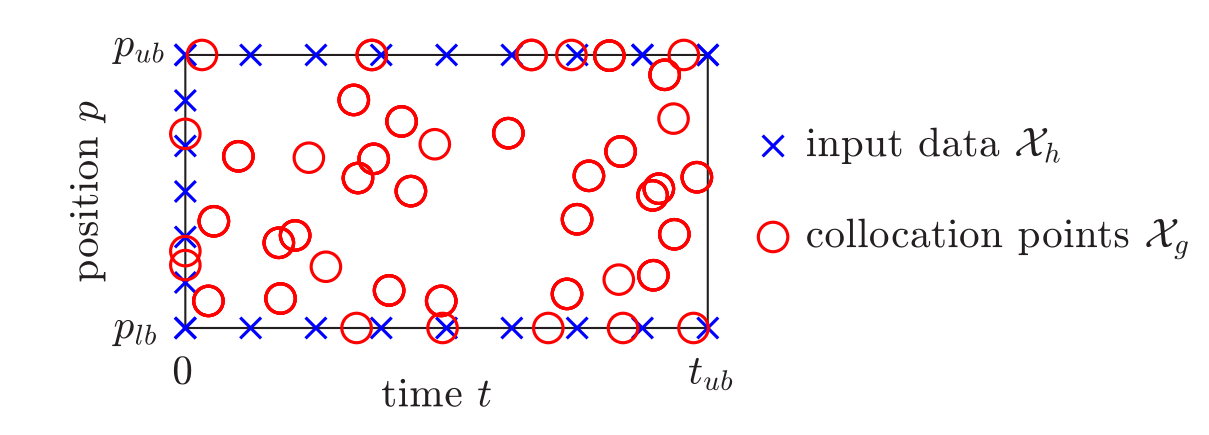
\includegraphics[width=0.8\textwidth]{img/space_time_grid.png}
    \caption{Space-Time grid points of the input data $\mathcal{X}_h$ and $\mathcal{X}_g$}
    \label{fig:space_time_grid}
\end{figure}   

\begin{align}
    \mathcal{X}_h &= \left\{
        \left(p_{h,1}, t_{h,1}\right),
        \cdots,
        \left(p_{h,i}, t_{h,i}\right),
        \cdots,
        \left(p_{h,n_h}, t_{h,n_h}\right)
    \right\}\\
    \mathcal{Y}_h &= \left\{
        h\left(p_{h,1}, t_{h,1}\right),
        \cdots,
        h\left(p_{h,i}, t_{h,i}\right),
        \cdots,
        h\left(p_{h,n_h}, t_{h,n_h}\right)
    \right\}
\end{align}

\begin{equation}
    \mathcal{X}_g = \left\{
        \left(p_{g,1}, t_{g,1}\right),
        \cdots,
        \left(p_{g,i}, t_{g,i}\right),
        \cdots,
        \left(p_{g,n_g}, t_{g,n_g}\right)
    \right\}
\end{equation}
\end{frame}

\begin{frame}{Fitting Procedure}
\framesubtitle{Loss Function}

The loss functions is divided into two parts:

\begin{itemize}
    \item Loss function for the boundary conditions:
    \begin{equation}
        \mathcal{L}_h (\mathcal{X}_h, \mathcal{Y}_h, \psi) = \frac{1}{n_h} \sum_{i=1}^{n_h} \left| h(p_{h,i}, t_{h,i}) - \psi(p_{h,i}, t_{h,i})  \right|^2
    \end{equation}
    \item Loss function for the PDE:
    \begin{equation}
        \mathcal{L}_g (\mathcal{X}_g, \psi)= \frac{1}{n_g} \sum_{i=1}^{n_g} \left| \frac{\partial }{\partial t}\psi(p_{g,i}, t_{g, i}) + \mathcal{F}(\psi(p_{g,i}, t_{g, i})) \right|^2
    \end{equation}
\end{itemize}
\end{frame}

\begin{frame}{Fitting Procedure}
\framesubtitle{Total Loss Function}

The total loss function is given by:

\begin{equation}
    \mathcal{L}(\mathcal{X}_h, \mathcal{Y}_h,\mathcal{X}_g, \psi) = \mathcal{L}_h (\mathcal{X}_h, \mathcal{Y}_h, \psi) + \mathcal{L}_g (\mathcal{X}_g, \psi)
\end{equation}

And we aim to minimize it with respect to the parameters of the neural network $\psi$.

\end{frame}

\begin{frame}{Limitations}
    
The PINN method is only suitable for autonomous PDEs in a bounded space-time domain.

Arnold and King (2021) propose a state-space model based on PINNs. This approach enables dynamic system control and state estimation, and is suitable for applying the Extended Kalman Filter (EKF), using automatic differentiation to address system non-linearities.


{\tiny Arnold, Florian, and Rudibert King. "State-Space Modeling for Control Based on Physics-Informed Neural Networks." \textit{Engineering Applications of Artificial Intelligence} 101 (2021): 104195. Elsevier.}
\end{frame}

\begin{frame}{State-Space Modeling}

The general State-Space model is given by:

\begin{align}
x_{k+1}  &= f(x_k, u_k) \quad (\text{State Equation})\\
y_k &= z(x_k, u_k) \quad (\text{Measurement Equation})
\end{align}

where $x_k$ is the state, $u_k$ is the control input, and $y_k$ is the measurement at time $k$.

How can we define the state of the system in terms of the PDE solution $h(p, t)$?
\end{frame}

\begin{frame}{State-Space Modeling}
\framesubtitle{State Definition}

\begin{itemize}
    \item The PDE solution $h(p, t) \approx \psi(p, t)$ describes the course of a physical quantity over time and space (represented by color in the figure).
    \begin{itemize}
        \item The physical quantity has a different evolution over time depending on the position $p$ in the space domain.
    \end{itemize}
\end{itemize}

\begin{figure}[H]
    \centering
    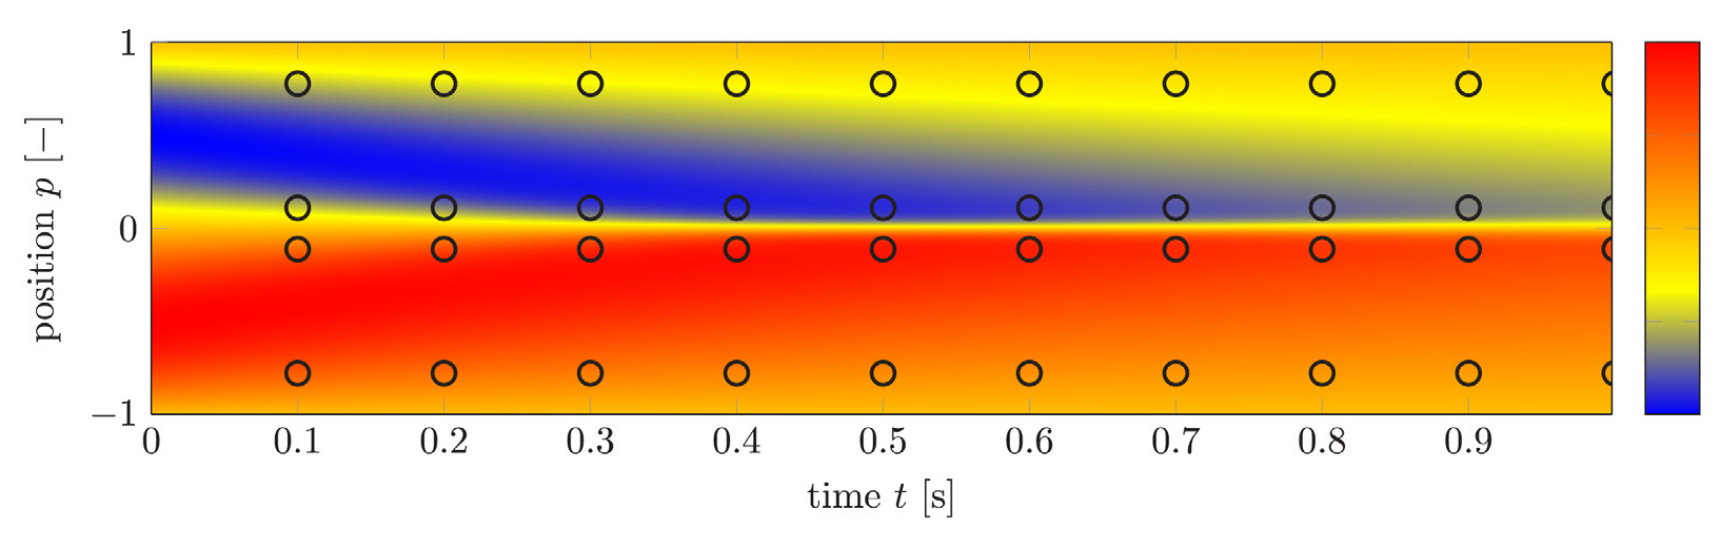
\includegraphics[width=0.8\textwidth]{img/state_space_time.png}
    \caption{Evolution of the system over time for different positions $p$ in the space domain.}
\end{figure}
\end{frame}

\begin{frame}{State-Space Modeling}
\framesubtitle{State Definition}
\begin{figure}[H]
    \centering
    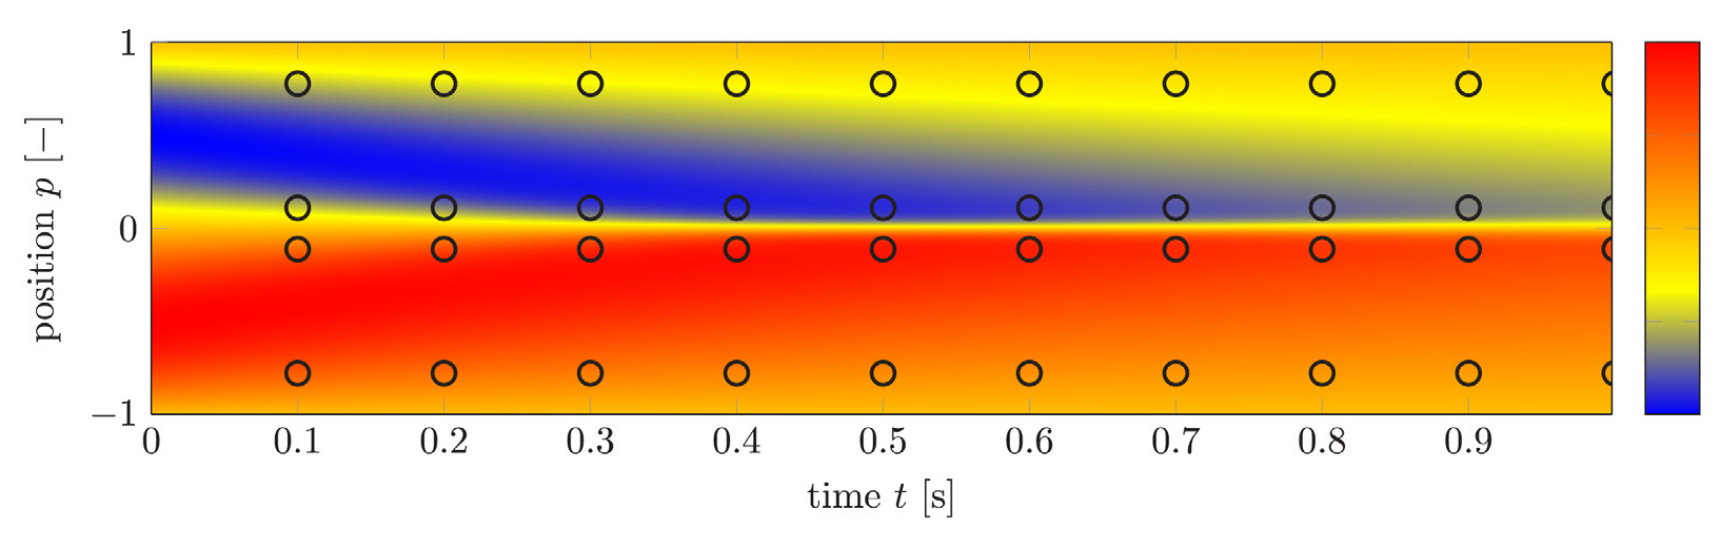
\includegraphics[width=0.5\textwidth]{img/state_space_time.png}
\end{figure}

\begin{itemize}
\item Arnold and King (2021) propose to define the state $x_t$ of the system as the PDE solution $h(p, t)$ at a specific position $p_x$ in the space domain at time $t$.
\end{itemize}
\end{frame}

\begin{frame}{State-Space Modeling}
\framesubtitle{State Definition}

For example, for a set $\mathcal{P}$ of positions in the space domain:
\begin{align}
\mathcal{P} &= \{p_{x,1},\cdots, p_{x,i}, \cdots, p_{x,n_x}\}
\end{align}

the initial conditions ($t=0$) of the state-space model are given by:

\begin{align}
x_0 = \left[h(p_{x,1}, 0), \cdots,h(p_{x,i}, 0), \cdots, h(p_{x,n_x}, 0) \right]^T
\end{align}

In fact, the initial conditions are a continuous on the space domain. 
\end{frame}

\begin{frame}{State-Space Modeling}
\framesubtitle{Fitting (First Approach)}

From the PINN fitting procedure, we have the following boundary conditions:

\begin{align*}
    \mathcal{X}_h &= \left\{
        \left(p_{h,1}, t_{h,1}\right),
        \cdots,
        \left(p_{h,i}, t_{h,i}\right),
        \cdots,
        \left(p_{h,n_h}, t_{h,n_h}\right)
    \right\}\\
    \mathcal{Y}_h &= \left\{
        h\left(p_{h,1}, t_{h,1}\right),
        \cdots,
        h\left(p_{h,i}, t_{h,i}\right),
        \cdots,
        h\left(p_{h,n_h}, t_{h,n_h}\right)
    \right\}
\end{align*}

It contains the initial conditions of the state-space model. We can separate these initial conditions from the boundary conditions:

\begin{align}
    \mathcal{X}_0 &= \left\{
        (p_{h,i}, t_{h,i}) \in \mathcal{X}_h: t_{h,i} = 0
    \right\}\\
    \mathcal{Y}_0 &= \left\{
        h(p_{h,i}, t_{h,i}) \in \mathcal{Y}_h: t_{h,i} = 0
    \right\}\\
    \bar{\mathcal{X}}_h &= \mathcal{X}_h \setminus \mathcal{X}_0\\
    \bar{\mathcal{Y}}_h &= \mathcal{Y}_h \setminus \mathcal{Y}_0 
\end{align}
\end{frame}

\begin{frame}{State-Space Modeling}
\framesubtitle{Fitting (First Approach), First Iteration}

Our goal (in a first iteration) is to select the neural network $\psi_0(p, t)$ that minimizes the loss function:

\begin{align*}
    \mathcal{L}(\mathcal{X}_0, \mathcal{Y}_0, \bar{\mathcal{X}}_h, \bar{\mathcal{Y}}_h,\mathcal{X}_g, \psi_0) =& \mathcal{L}_0 (\mathcal{X}_0, \mathcal{Y}_0, \psi_0) \\
    +& \mathcal{L}_h (\bar{\mathcal{X}}_h, \bar{\mathcal{Y}}_h, \psi_0) \\
    +& \mathcal{L}_g (\mathcal{X}_g, \psi_0)
\end{align*}

Where:
\begin{equation}
    \mathcal{L}_0 (\mathcal{X}_0, \mathcal{Y}_0, \psi_0) = \frac{1}{|\mathcal{X}_0|} \sum_{(p_{h,i}, t) \in \mathcal{X}_0} \left| h(p_{h,i}, t_{h,i}) - \psi_0(p_{h,i}, t_{h,i})  \right|^2
\end{equation}

At this point, the training of $\psi_0$ is equivalent to the PINN in the original setup. 

\end{frame}

\begin{frame}{State-Space Modeling}
\framesubtitle{Fitting (First Approach), Second Iteration}

In a second iteration, we aim to train the neural network $\psi_1(p, t + \Delta t)$ to minimize the loss function:

\begin{align*}
    \mathcal{L}(\mathcal{X}_0, \bar{\mathcal{X}}_h, \bar{\mathcal{Y}}_h,\mathcal{X}_g, \psi_0) =& \mathcal{L}_1 (\mathcal{X}_0, \psi_1) \\
    +& \mathcal{L}_h (\bar{\mathcal{X}}_h, \bar{\mathcal{Y}}_h, \psi_0) \\
    +& \mathcal{L}_g (\mathcal{X}_g, \psi_0)
\end{align*}

Where:
\begin{equation}
    \mathcal{L}_1 (\mathcal{X}_0, \psi_1) = \frac{1}{|\mathcal{X}_0|} \sum_{(p_{h,i}, t) \in \mathcal{X}_0} \left| \psi_0(p_{h,i}, t_{h,i} + \Delta t) - \psi_1(p_{h,i}, t_{h,i} + \Delta t)  \right|^2
\end{equation}

\end{frame}

\begin{frame}{State-Space Modeling}
\framesubtitle{Fitting (First Approach), Other Interations}

the algorithm is repeated for each time step $t_k = k \Delta t$ until the final time $t_{ub}$, fitting a total of $t_{ub}/\Delta t$ neural networks $\psi_k(p, t)$.

\end{frame}

\begin{frame}{State-Space Modeling}
\framesubtitle{Fitting (First Approach), Limitations}

\begin{itemize}
    \item Computationally expensive.
    \item The algorithm should be repeated for a discretization of the possible control inputs $u_k$.
    \item Not suitable for real time control, since the training of a neural network $\psi_k$ is required for each time step $t_k$.
\end{itemize}

\end{frame}

\begin{frame}{State-Space Modeling}
\framesubtitle{Fitting (Second Approach)}

Instead of fitting a neural network $\psi_k(p, t)$ for each time step $t_k$, a unique neural network:

\begin{equation}
h(p, t)_{x_k} \approx \psi(p, t, x_k)
\end{equation}

can be trained for arbitrary initial conditions $x_k$.

\end{frame}

\begin{frame}{State-Space Modeling}
\framesubtitle{Fitting (Second Approach)}

Instead of fitting a neural network $\psi_k(p, t)$ for each time step $t_k$, a unique neural network:

\begin{equation}
h(p, t)_{x_k} \approx \psi(p, t, x_k)
\end{equation}

can be trained for arbitrary initial conditions $x_k$.

\end{frame}

\begin{frame}{State-Space Modeling}
\framesubtitle{Fitting (Second Approach)}

\begin{itemize}
    \item The neural network $\psi(p, t, x_k)$ now require an additional set of states $x_k$ for the fitting.
    \item The neural network $\psi(p, t, x_k)$ in only suitable for a path $u_k$ of control inputs.
    \begin{itemize}
        \item At least two neural networks $\psi_{\bar{u}}(p, t, x_k)$ and $\psi_{\underbar{u}}(p, t, x_k)$ have to be trained to compare the influence of different control inputs.
    \end{itemize}
\end{itemize}

\end{frame}

\begin{frame}{State-Space Modeling}
\framesubtitle{Fitting (Second Approach)}

With this training, the original state-space model can be replaced by:

\begin{align}
x_{k+1} &= \left[\begin{matrix}
I_u \left(\psi_{\bar{u}}(p_{x,1}, \Delta t, x_k), \psi_{\underbar{u}}(p_{x,1}, \Delta t, x_k)\right) \\
\vdots\\
I_u \left(\psi_{\bar{u}}(p_{x,i}, \Delta t, x_k), \psi_{\underbar{u}}(p_{x,i}, \Delta t, x_k)\right) \\
\vdots\\
I_u \left(\psi_{\bar{u}}(p_{x,n_x}, \Delta t, x_k), \psi_{\underbar{u}}(p_{x,n_x}, \Delta t, x_k)\right) \\
\end{matrix}
\right]\\
y_k &= z(x_k, u_k)
\end{align}

\end{frame}
